% *********************************************************************
% © 2021 Jeremy Sylvestre
%
% Permission is granted to copy, distribute and/or modify this document
% under the terms of the GNU Free Documentation License, Version 1.3 or
% any later version published by the Free Software Foundation; with no
% Invariant Sections, no Front-Cover Texts, and no Back-Cover Texts. A
% copy of the license is included in the appendix entitled “GNU Free
% Documentation License” that appears in the output document of this
% PreTeXt source code. All trademarks™ are the registered® marks of
% their respective owners.
%
% *********************************************************************

\newcommand*{\xmin}{0.5}
\newcommand*{\xmax}{6}
\newcommand*{\ymin}{-2.5}
\newcommand*{\ymax}{5}
\newcommand*{\func}{\x * \x * \x * \x / 4 - 3 * \x * \x * \x + 23 * \x * \x / 2 - 14 * \x + 3}

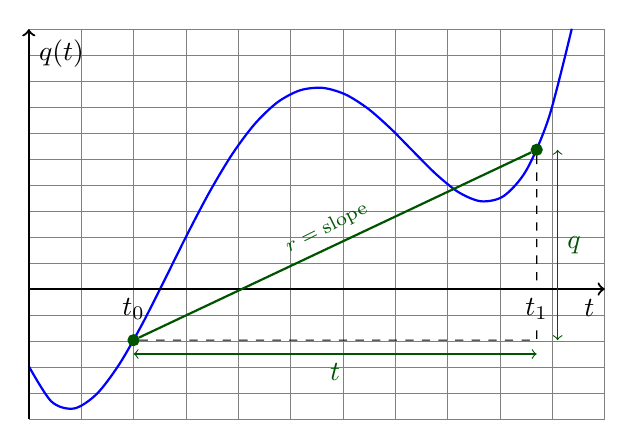
\begin{tikzpicture}
[
	closedpt/.style={circle,draw,fill,inner sep=0pt,minimum size=4pt},
	openpt/.style={circle,draw,inner sep=0pt,minimum size=4pt},
	xscale=1.33,
	yscale=0.66
]

	% grid
	\foreach \x in {0.5,1,1.5,...,6} {
		\draw[very thin,gray] (\x,\ymin) -- (\x,\ymax);
	}
	\foreach \y in {-2.5,-2,-1.5,...,5} {
		\draw[very thin,gray] (\xmin,\y) -- (\xmax,\y);
	}

	% example graph
	\draw[thick, blue, domain=0.5:5.685, smooth, thick] plot (\x,{\func});

	% axes
	\draw[->,thick] (\xmin,0) -- (\xmax,0) node[below left] {$t$};
	\draw[->,thick] (0.5,\ymin) -- (0.5,\ymax) node[below right] {$q(t)$};

	\node[closedpt, green!33!black] at (1.5,-0.984) (start) {};
	\node[closedpt, green!33!black] at (5.35,2.68) (end) {};

	\draw[green!33!black, thick] (start) -- node[above,sloped,rotate=-17] {$\scriptstyle \avg{r} \; = \; \mathrm{slope}$} (end);
	\draw[dashed,thin] (end) -- (5.35,0);

	\node[below] at (1.5,0) {$t_0$};
	\node[below] at (5.35,0) (t1) {$t_1$};

	\draw[dashed] (start) -- (5.35, -0.984) -- (t1);

	\draw[green!33!black,<->] (1.5,-1.25) -- node[below] {$\change{t}$} (5.35,-1.25);
	\draw[green!33!black,<->] (5.55,2.68) -- node[right] {$\change{q}$} (5.55,-0.984);

\end{tikzpicture}
